\chapter{推論統計:假說檢定}

    推論統計的目的是了解背後母群體的特性,或更精確地來說,背後母群體的參數取值狀況。例如在民意調查中,我們感興趣的母體參數是全民政策支持率 $p$,而推論統計希望可以藉由有限的抽樣樣本來了解 $p$ 的取值。推論統計的方法主要可以分成兩大分支:估計以及假說檢定。估計採取的策略較為直接,希望可以從樣本計算出一個估計值(點估計)或估計區間(區間估計),來描述 $p$ 的可能取值。假說檢定採取的則是科學中假說-預測-證偽的典範,首先提出假說,並根據假說預測觀察資料應有的特徵,而後實際檢視資料是否\textbf{不符}該特徵而將假說\textbf{證偽}。本章將探討如何將上述流程具象化為統計檢定的步驟,其中會大量用到條件機率以及抽樣分布的概念,希望讀者能夠融會貫通。
    
    \begin{introduction}[第 \thechapter 章學習目標]
        \item 建構假說檢定的基本架構
        \item 虛無假說、對立假說、虛無分布及顯著水準的意義
        \item 了解如何解釋 $p$ 值
        \item 常見情境的母體平均單樣本檢定
        \item 信賴區間與檢定的關係
        \item 檢定的型一錯誤率、型二錯誤率、檢定力與樣本數計算
    \end{introduction}

\section{假說檢定的基本架構}

    在進入假說檢定的架構前,我們先考慮以下的情境:假設某 A 同學宣稱他有猜拳的天賦,贏拳的機率高於一般認為的 1/3。你不相信並想要挑戰他。於是,你跟他猜了五次拳,結果他贏了四次。這時候你想著,如果他猜拳能力只是一般的 1/3,那麽猜五次裡面贏四次以上的機率是(根據我們學到的二項分布機率質量函數)
    \[\binom{5}{4} \cdot \Big(\frac{1}{3}\Big)^4 \cdot \frac{2}{3} + \binom{5}{5} \cdot \Big(\frac{1}{3}\Big)^5 \approx 0.0453\]
    也就是說,如果他只是一般的猜拳者,那麼他贏得這麼徹底的機率只有約 $4.5 \%$。你覺得這樣的機率太低了,不太可能發生。因此,你認為 A 同學的確有一些猜拳的技術,讓他的猜拳贏拳機率比 1/3 還要高。

    上述的流程雖然十分簡單,但已經蘊含了假說檢定的基本架構。首先,我們需要有一個想\textbf{證偽}的命題,並把這個命題量化成為一個假說。這個假說建立的目的是要被證偽,因此被稱為\textit{虛無假說} (null hypothesis),符號上通常記為 $H_0$。上述的情境中,我們想要證偽的命題是「A 同學的猜拳能力等同一般人」,量化後的虛無假說即為「A 同學猜拳贏拳的機率 $p = 1/3$」。有了虛無假說後,我們還需要建立虛無假說的對立面,也就是將虛無假說證偽後希望得到的結論。這個對立的假說被稱為\textit{對立假說} (alternative hypothesis),符號上通常記為 $H_1$ 或 $H_a$。上述情境中,我們希望證偽虛無假說後,能夠認定 A 同學真的有猜拳的天賦,因此對立假說是「A 同學猜拳贏拳的機率 $p > 1/3$」(注意到對立假說不一定要是虛無假說的補集)。我們通常會將這兩個假說並陳如下(令 $p$ 為 A 同學猜拳贏拳的機率):
    \begin{align*}
        H_0: \;&p = 1/3\\
        H_1: \;&p > 1/3
    \end{align*}
    訂好假說後,我們要判斷資料是否\textbf{不符合}虛無假說下的情境,以決定是否能證偽虛無假說。為了方便判斷,我們會利用資料計算出一個\textit{測驗統計量},這個測驗統計量通常會儘量滿足兩個特點:(1) 我們知道該統計量在虛無假說下的抽樣分布,這個分布被稱為虛無分布 (null distribution) (2) 當對立假說成立時,該統計量的取值落在虛無分布較極端的位置,例如偏大、偏小、或是在分布的兩端。需要這兩點的原因在於,我們希望算出測驗統計量時,可以用方向來判斷統計量是否偏離虛無假說並偏向對立假說,並且能用虛無分布來量化該統計量有多極端。在上述的例子中,我們的測驗統計量是猜拳五次後 A 同學贏的總次數,我們簡單記為 $T$。我們知道 $T$ 在虛無假說下服從一個次數參數為 5、機率參數為 1/3 的二項分布。此分佈即虛無分布,如圖 \ref{fig:null_dist_binom}。而且我們還知道,當對立假說成立時,$T$ 的取值應該會偏大。因此,$T$ 符合我們對於測驗統計量的要求。

    \begin{figure}[htbp]
        \centering
        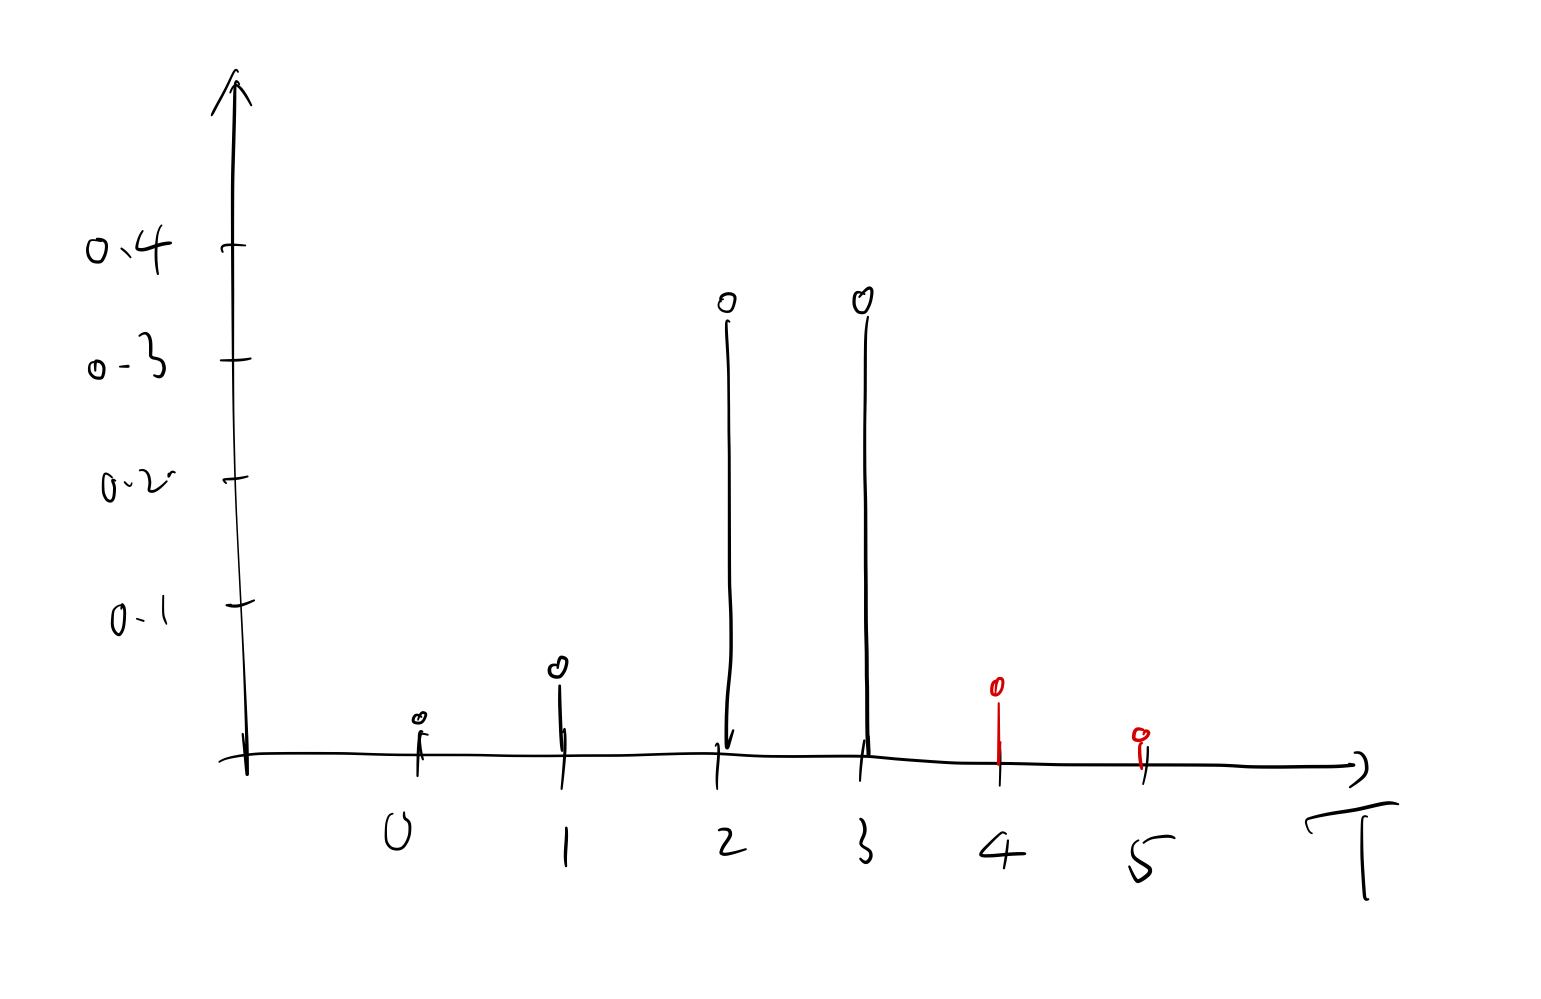
\includegraphics[width=0.7\textwidth]{figures/06-Hypothesis_testing/null_dist_binom.jpeg}
        \caption{猜拳實驗假說檢定的虛無分佈}
        \label{fig:null_dist_binom}
    \end{figure}
 
    接下來,我們要用虛無分布來量化我們觀察到的 $T=4$ 是否足夠極端。我們量化的方法是計算「在虛無分布下,$T$ 的取值和觀察值一樣極端,或比觀察值還要極端的機率」,其中極端的定義是接近對立假說的取值。例如上述情況中,我們知道 $T$ 取值越大,代表贏拳次數越多,也就越接近我們的對立假說。因此,我們要計算「在虛無分布下,$T$ 的取值大於或等於 $4$ 的機率」,也就是圖 \ref{fig:null_dist_binom}中兩個紅色的機率相加,我們之前算出是 0.0453。這個機率我們稱為檢定的 $p$\textit{值} ($p$-value)。該值越小,代表測驗統計量處於越極端的的位置,也就隱含著虛無假設越不可能成立。

    在上述的例子中,我們認為 $p$ 值 0.0453「夠小」,足以證偽虛無假設而接受對立假設 $p > 1/3$,也就是 A 同學有優於常人的猜拳能力。然而,有些人可能認為 0.0453 不夠小,仍然無法排除是 A 同學只是運氣好贏了四次。因此,我們需要訂定一個判準來決定怎麼樣子的 $p$ 值叫做「夠小」。這個判準通常被稱為\textit{顯著水準} (significance level),符號寫作 $\alpha$。當 $p \le \alpha$ 時,我們就認為 $p$ 值夠小,並稱檢定\textit{顯著} (significant),可以拒絕虛無假說並接受對立假設。這種檢定的方法我們稱為 \textbf{$p$ 值法}。舉例來說,上述的例子我們可以設定顯著水準為 0.05,並注意到 $p = 0.0453 \le 0.05$,因此「在顯著水準 0.05 下,我們拒絕虛無假說,並得出 A 同學有\textit{統計上顯著} (statistically significant) 優於常人的猜拳能力」。但若設定顯著水準為 0.01,因為 $p = 0.0435 > 0.01$,只能說「在顯著水準 0.01 下,我們\textbf{無法拒絕}虛無假說,因此\textbf{沒有足夠證據證明} A 同學的猜拳能力優於常人」。

    從圖 \ref{fig:null_dist_binom} 可以看出,如果我們設定 $\alpha = 0.05$,由於我們只有在 $p$ 值小於 $0.05$ 時才拒絕虛無假說,因此只有 $T \ge 4$ 時才會拒絕虛無假說($\PP(T \ge 3 | H_0) = 0.5 \ge 0.05$)。這個 $T \ge 4$ 也被稱為檢定的\textit{拒絕域} (rejection region),而其邊界 $T=4$ 則是檢定的\textit{臨界值} (critical value)。如果我們可以先找到拒絕域 $T \ge 4$,就可以在不用算出 $p$ 值的情況下,僅憑檢定統計量 $T$ 的觀察值逕行決定是否拒絕虛無假說。這種檢定方法我們稱為\textbf{拒絕域法}。
    
    拒絕域的建構方法如下:首先我們需要根據虛無假說及對立假說的相對關係決定拒絕域的型態。例如上述例子中,我們知道 $T$ 越大,證據越偏向對立假說,因此拒絕域的型態應該型如 $T \ge c$,其中 $c$ 是待定的常數。然後,我們需要找到符合 $\PP(T \ge c | H_0) \le \alpha$ 的條件下,讓拒絕域最大化的 $c$。其中 $\PP(T \ge c | H_0)$ 代表「在虛無假說正確下拒絕虛無假說」的機率,也就是「冤枉了虛無假說」的機率。這種「冤枉虛無假說」事件也被稱為犯下\textit{型一錯誤} (type I error)。換言之,我們希望在控制型一錯誤率不高於顯著水準的情況下,盡可能地擴大拒絕域。在上述的例子中,若將顯著水準 $\alpha$ 設定為 0.05,則 $c$ 最小的可行取值為 $4$,因為 $\PP(T \ge 4 | H_0) = 0.0453 \le 0.05, \PP(T \ge 3 | H_0) = 0.5 > 0.05$。因此,顯著水準 0.05 下的拒絕域為 $T \ge 4$,臨界值為 $4$。

    從前面的討論可以看到,統計檢定顯著與否有一大部分取決於顯著水準 $\alpha$。為了避免做檢定時看到檢定統計量觀察值才移動顯著水準,進而操弄檢定的顯著性,一般我們會在進行檢定前就設定好顯著水準。在生醫統計中最常使用的顯著水準為 0.05,但在一些特別的檢定也可能設定為 0.1 或 0.01。事實上,0.05 的設定完全沒有科學根據,僅是根據 Ronald Fisher 在一篇文章寫到「... Personally, the writer prefers to set a low standard of significance at the 5 per cent. point, ...」,後人效仿後漸漸成為約定俗成。

    最後,我們把統計檢定的步驟作成如圖 \ref{fig:hypothesis_flowchart} 的流程圖。

    \bigskip

    \begin{custom}{思考}
       如果把顯著水準提高,拒絕域應該會變寬或是變窄?
    \end{custom}

    \begin{figure}
        \begin{center}
            \begin{tikzpicture}[node distance=1.5cm]
                \node (one) [rnd] {1. 寫出欲證偽的命題,以及與該命題對立、證偽後欲接受的命題};
                \node (two) [rnd, below of = one] {2. 將命題量化為虛無假說與對立假說};
                \node (three) [rnd, below of = two] {3. 訂定顯著水準 $\alpha$};
                \node (four) [rnd, below of = three] {4. 選定檢定統計量 $T$ 並計算數值};
                \node (five) [below of = four, yshift = -1cm] {};
                \node (six) [below of = five] {};
                \node (seven) [below of = six, yshift = -1cm] {};
                \node (fiveone) [rnd, left of = five, xshift = -2cm] {5-1. 根據 $\alpha$ 計算臨界值與拒絕域};
                \node (sixone) [rnd, below of = fiveone] {6-1. 判定 $T$ 是否落在拒絕域};
                \node (fivetwo) [rnd, right of = five, xshift = 2cm] {5-2. 計算 $p$ 值};
                \node (sixtwo) [rnd, below of = fivetwo] {6-2. 判定是否 $p \le \alpha$};
                \node (sevenr) [rnd, below of = sixone, yshift = -1cm] {7a. 拒絕虛無假說,接受對立假說};
                \node (sevena) [rnd, below of = sixtwo, yshift = -1cm] {7b. 無法拒絕虛無假說};
                \node (eight) [rnd, below of = seven] {8. 撰寫結論};
                \draw [arrow] (one) -- (two);
                \draw [arrow] (two) -- (three);
                \draw [arrow] (three) -- (four);
                \draw [arrow] (four) -- node[anchor=east] {拒絕域法}(fiveone);
                \draw [arrow] (four) -- node[anchor=west] {$p$值法}(fivetwo);
                \draw [arrow] (fiveone) -- (sixone);
                \draw [arrow] (fivetwo) -- (sixtwo);
                \draw [arrow] (sixone) -- node[anchor=east] {是} (sevenr);
                \draw [arrow] (sixtwo) -- node[anchor=south east] {否} (sevenr);
                \draw [arrow] (sixone) -- node[anchor=south west] {是} (sevena);
                \draw [arrow] (sixtwo) -- node[anchor=west] {否} (sevena);
                \draw [arrow] (sevenr) -- (eight);
                \draw [arrow] (sevena) -- (eight);
            \end{tikzpicture}
        \end{center}
        \caption{假說檢定流程圖}
        \label{fig:hypothesis_flowchart}
    \end{figure}

\section{母體平均的單樣本檢定:母體為常態分布且變異數已知}
    有了上一節的框架後,我們可以來看幾個情境下,針對母體平均的統計檢定。假設已知母體為常態分布且變異數已知為 $\sigma^2$,抽取樣本數為 $n$ 的樣本並得到樣本平均為 $\bar{X}$。我們分成三種情況討論(母體平均參數以 $\mu$ 表示):

    \noindent\underline{\textbf{右尾檢定}}

    若假說形如 $H_0: \; \mu = \mu_0 \; ; \; H_1: \; \mu > \mu_0$,則在虛無假說下,根據樣本平均的性質:
    \[\bar{X} \sim \NN\Big(\mu_0, \frac{\sigma^2}{n}\Big)\]
    因此我們可以把 $\bar{X}$ 作 $z$ 轉換當成檢定統計量,其虛無分布為標準常態分佈:
    \[Z = \frac{\bar{X}-\mu_0}{\sigma/\sqrt{n}} \sim \ZZ\]
    設定顯著水準為 $\alpha$ 的情況下,我們可以用 $p$ 值法或拒絕域法來建構檢定:

    \noindent \underline{$p$ 值法}:當對立假說為真時,$\bar{X}$ 的期望值 $\mu$ 會比 $\mu_0$ 來得大,因此 $Z$ 偏大的方向是比較「極端」的方向。根據 $p$ 值的定義可以寫出
    \[p = \PP(\ZZ \ge Z)\]
    即對應到圖\ref{fig:one_sample_z}左圖紅色的面積。此時若 $p \le \alpha$ 則拒絕虛無假說、接受對立假說;反之則無法拒絕虛無假說。
    
    \noindent \underline{拒絕域法}:因為 $Z$ 值偏大的方向是傾向對立假說,所以拒絕域應該形如 $Z \ge c$。此時我們希望控制型一錯誤率在 $\alpha$ 以內,因此需要
    \[\PP(Z \ge c|H_0) \le \alpha\]
    根據 $Z$ 的虛無分布,上述等價於
    \[\PP(\ZZ \ge c) \le \alpha\]
    滿足這個不等式最小的 $c$ 即為 $z_\alpha$(因為 $\PP(\ZZ \ge z_\alpha) = \alpha$),因此本檢定的拒絕區為 $Z \ge z_\alpha$,統計量臨界值為 $z_\alpha$,即對應到圖\ref{fig:one_sample_z}右圖紅色的切點,其中紅色面積為$\alpha$。可以看到拒絕區具有右邊的尾巴,所以這組虛無假說對應的檢定又稱為右尾檢定。若檢定統計量落在拒絕區,則拒絕虛無假說、接受對立假說;反之則無法拒絕虛無假說。

    \noindent\underline{\textbf{左尾檢定}}

    若假說形如 $H_0: \; \mu = \mu_0 \; ; \; H_1: \; \mu < \mu_0$,則檢定統計量和檢定統計量的虛無分佈均和右尾檢定相同,差別僅在於 $p$ 值法和拒絕域法的定義方向:

    \noindent \underline{$p$ 值法}:當對立假說為真時,$\bar{X}$ 的期望值 $\mu$ 會比 $\mu_0$ 來得小,因此 $Z$ 偏小的方向是比較「極端」的方向。根據 $p$ 值的定義可以寫出
    \[p = \PP(\ZZ \le Z)\]
    即對應到圖\ref{fig:one_sample_z}左圖黑色的面積。此時若 $p \le \alpha$ 則拒絕虛無假說、接受對立假說;反之則無法拒絕虛無假說。
    
    \noindent \underline{拒絕域法}:因為 $Z$ 值偏小的方向是傾向對立假說,所以拒絕域應該形如 $Z \le c$。經由相似的計算可得到拒絕區為 $Z \le -z_\alpha$,統計量臨界值為 $-z_\alpha$,即對應到圖\ref{fig:one_sample_z}右圖黑色的切點,其中黑色面積為$\alpha$。此拒絕區具有左邊的尾巴,所以這組虛無假說對應的檢定又稱為左尾檢定。若檢定統計量落在拒絕區,則拒絕虛無假說、接受對立假說;反之則無法拒絕虛無假說。

    \noindent\underline{\textbf{雙尾檢定}}

    若假說形如 $H_0: \; \mu = \mu_0 \; ; \; H_1: \; \mu \ne \mu_0$,則檢定統計量和檢定統計量的虛無分佈仍和右尾檢定相同,但 $p$ 值法和拒絕域法的定義方向則和前面兩個情境均不同。

    \noindent \underline{$p$ 值法}:當對立假說為真時,$\bar{X}$ 的期望值 $\mu$ 會往兩側遠離 $\mu_0$,因此 $Z$ 不論偏大或偏小都是「極端」的方向。且因為 $Z$ 的虛無分布期望值為零,$Z$ 和 $-Z$ 的極端程度是一樣的。如圖\ref{fig:one_sample_z}左圖所示。所以根據 $p$ 值的定義可以寫出
    \[p = \PP((\ZZ \ge |Z|)\cup(\ZZ \le -|Z|)) = 2\PP(\ZZ \ge |Z|)\]
    即對應到圖\ref{fig:one_sample_z}左圖藍色的面積。此時若 $p \le \alpha$ 則拒絕虛無假說、接受對立假說;反之則無法拒絕虛無假說。
    
    \noindent \underline{拒絕域法}:因為 $Z$ 值不論偏大或偏小均是傾向對立假說,而且 $Z$ 的虛無分布期望值為零,所以拒絕域應該形如 $(Z \ge c)\cup(Z \le -c)$,或可寫為$|Z| \ge c$。此時我們希望控制型一錯誤率在 $\alpha$ 以內,因此需要
    \[\PP(|Z| \ge c|H_0) \le \alpha\]
    根據 $Z$ 的虛無分布,上述等價於
    \[\PP(|\ZZ| \ge c) \le \alpha\]
    \[\PP(\ZZ \ge c) \le \alpha/2\]
    滿足這個不等式最小的 $c$ 即為 $z_{\alpha/2}$,因此本檢定的拒絕區為 $|Z| \ge z_{\alpha/2}$,統計量臨界值為 $\pm z_{\alpha/2}$,即對應到圖\ref{fig:one_sample_z}右圖藍色的切點,其中兩側藍色面積各為$\alpha/2$。此拒絕區兩邊均有尾巴,所以這組虛無假說對應的檢定又稱為雙尾檢定。若檢定統計量落在拒絕區,則拒絕虛無假說、接受對立假說;反之則無法拒絕虛無假說。

    \begin{figure}[htbp]
        \centering
        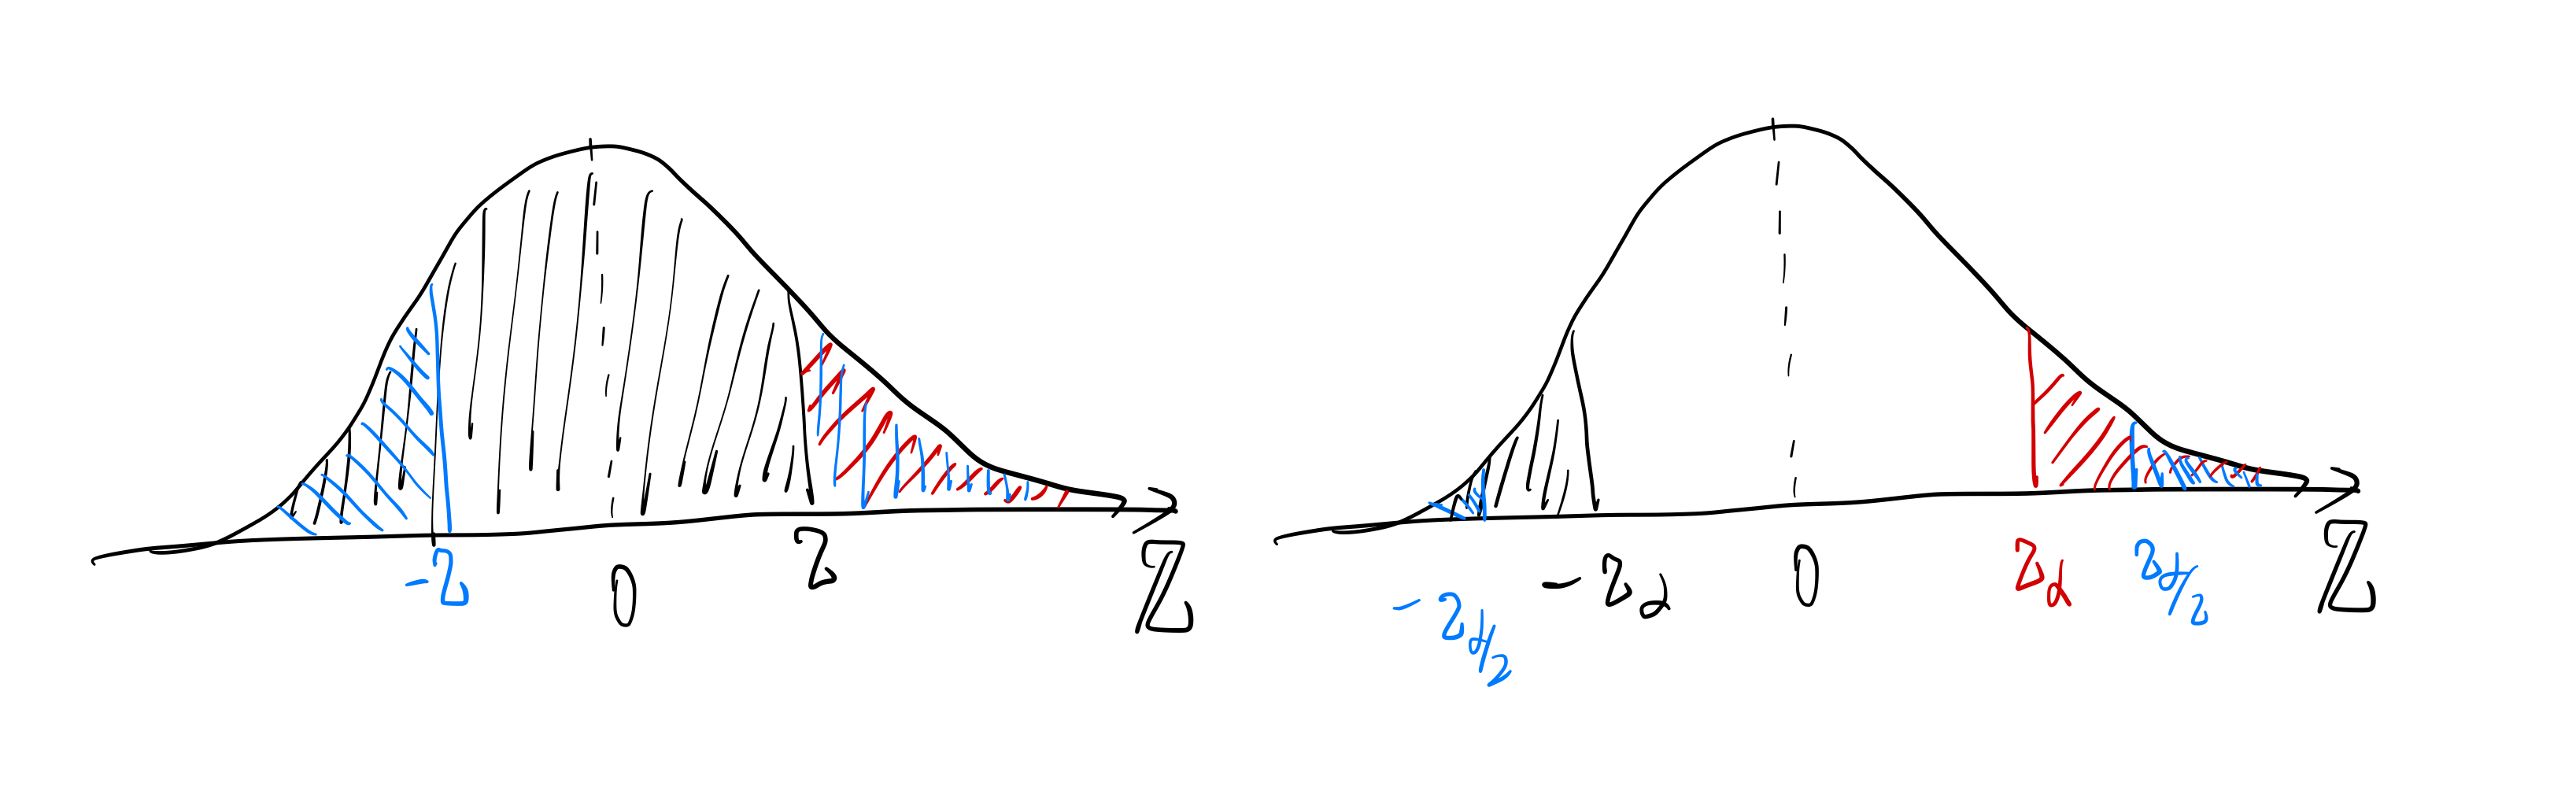
\includegraphics[width=\textwidth]{figures/06-Hypothesis_testing/one_sample_z.jpeg}
        \caption{母體為常態分布且變異數已知的母體平均檢定演示}
        \label{fig:one_sample_z}
    \end{figure}

    以下我們用表 \ref{tab:one_sample_z} 來整理母體為常態分布且變異數已知的母體平均檢定。由於此檢定只使用了一組樣本、是用 $Z$ 檢定統計量來建構、且統計量的虛無分布為標準常態分布($\ZZ$),因此此檢定亦稱為\textit{單樣本 Z 檢定} (One-sample Z test)。

    \begin{table}[htbp]
        \begin{center}
            \begin{tabular}{ccccc}
                \toprule
                虛無假說($H_0$) & 對立假說($H_1$) & 檢定統計量 & $p$ 值 & 拒絕區\\
                \hline
                \multirow{3}{*}{$\mu = \mu_0$} & $\mu > \mu_0$ & \multirow{3}{*}{$Z = \frac{\bar{X}-\mu_0}{\sigma/\sqrt{n}}$} & $\PP(\ZZ \ge Z)$ & $Z \ge z_{\alpha}$\\
                & $\mu < \mu_0$ & &$\PP(\ZZ \le Z)$&$Z \le -z_{\alpha}$\\
                & $\mu \ne \mu_0$ & &$2\times\PP(\ZZ \ge |Z|)$&$|Z| \ge z_{\alpha/2}$\\
                \bottomrule
            \end{tabular}
            \caption{母體為常態分布且變異數已知的母體平均檢定(單樣本 Z 檢定)\label{tab:one_sample_z}}
        \end{center}
    \end{table}
    
\section{母體平均的單樣本檢定:母體為常態分布且變異數未知}

    上一節我們假設了母體為常態分布且變異數已知,因此可以將樣本平均 $\bar{X}$ 進行 $z$ 轉換作為檢定統計量。然而,如果變異數未知,我們就無法直接作 $z$ 轉換了。幸運地是,在上一章我們提到的 $t$ 分布在這裡可以再度派上用場。假設已知母體為常態分布但變異數未知為,抽取樣本數為 $n$ 的樣本並得到樣本平均為 $\bar{X}$、樣本變異數為 $s^2$。我們仍然分成三種情況討論(母體平均參數以 $\mu$ 表示):

    \noindent\underline{\textbf{右尾檢定}}

    若假說形如 $H_0: \; \mu = \mu_0 \; ; \; H_1: \; \mu > \mu_0$,則在虛無假說下,根據$t$分布的定義:
    \[t = \frac{\bar{X}-\mu_0}{s/\sqrt{n}} \sim t_{n-1}\]
    設定顯著水準為 $\alpha$ 的情況下,我們用 $p$ 值法或拒絕域法來建構檢定:

    \noindent \underline{$p$ 值法}:當對立假說為真時,$\bar{X}$ 的期望值 $\mu$ 會比 $\mu_0$ 來得大,因此 $t$ 偏大的方向是比較「極端」的方向。根據 $p$ 值的定義可以寫出
    \[p = \PP(t_{n-1} \ge t)\]
    此時若 $p \le \alpha$ 則拒絕虛無假說、接受對立假說;反之則無法拒絕虛無假說。
    
    \noindent \underline{拒絕域法}:因為 $t$ 值偏大的方向是傾向對立假說,所以拒絕域應該形如 $t \ge c$。此時我們希望控制型一錯誤率在 $\alpha$ 以內,因此需要
    \[\PP(t \ge c|H_0) \le \alpha\]
    根據 $t$ 的虛無分布,上述等價於
    \[\PP(t_{n-1} \ge c) \le \alpha\]
    滿足這個不等式最小的 $c$ 為 $t_{n-1,\alpha}$(因為 $\PP(t_{n-1} \ge t_{n-1,\alpha}) = \alpha$),因此本檢定的拒絕區為 $t \ge t_{n-1,\alpha}$,統計量臨界值為 $t_{n-1,\alpha}$。若檢定統計量落在拒絕區,則拒絕虛無假說、接受對立假說;反之則無法拒絕虛無假說。

    \noindent\underline{\textbf{左尾檢定}}

    若假說形如 $H_0: \; \mu = \mu_0 \; ; \; H_1: \; \mu < \mu_0$,則檢定統計量和檢定統計量的虛無分佈均和右尾檢定相同,差別僅在於 $p$ 值法和拒絕域法的定義方向:

    \noindent \underline{$p$ 值法}:當對立假說為真時,$\bar{X}$ 的期望值 $\mu$ 會比 $\mu_0$ 來得小,因此 $t$ 偏小的方向是比較「極端」的方向。根據 $p$ 值的定義可以寫出
    \[p = \PP(t_{n-1} \le t)\]
    此時若 $p \le \alpha$ 則拒絕虛無假說、接受對立假說;反之則無法拒絕虛無假說。
    
    \noindent \underline{拒絕域法}:因為 $t$ 值偏小的方向是傾向對立假說,所以拒絕域應該形如 $t \le c$。經由相似的計算可得到拒絕區為 $t \le -t_{n-1,\alpha}$,統計量臨界值為 $-t_{n-1,\alpha}$。若檢定統計量落在拒絕區,則拒絕虛無假說、接受對立假說;反之則無法拒絕虛無假說。

    \noindent\underline{\textbf{雙尾檢定}}

    若假說形如 $H_0: \; \mu = \mu_0 \; ; \; H_1: \; \mu \ne \mu_0$,則檢定統計量和檢定統計量的虛無分佈仍和右尾檢定相同,但 $p$ 值法和拒絕域法的定義方向則和前面兩個情境均不同。

    \noindent \underline{$p$ 值法}:當對立假說為真時,$\bar{X}$ 的期望值 $\mu$ 會往兩側遠離 $\mu_0$,因此 $t$ 不論偏大或偏小都是「極端」的方向。且因為 $t$ 的虛無分布期望值為零,$t$ 和 $-t$ 的極端程度是一樣的。所以根據 $p$ 值的定義可以寫出
    \[p = \PP((t_{n-1} \ge |t|)\cup(t_{n-1} \le -|t|)) = 2\PP(t_{n-1} \ge |t|)\]
    此時若 $p \le \alpha$ 則拒絕虛無假說、接受對立假說;反之則無法拒絕虛無假說。
    
    \noindent \underline{拒絕域法}:因為 $t$ 值不論偏大或偏小均是傾向對立假說,而且 $t$ 的虛無分布期望值為零,所以拒絕域應該形如 $(t \ge c)\cup(t \le -c)$,或可寫為$|t| \ge c$。此時我們希望控制型一錯誤率在 $\alpha$ 以內,因此需要
    \[\PP(|t| \ge c|H_0) \le \alpha\]
    根據 $t$ 的虛無分布,上述等價於
    \[\PP(|t_{n-1}| \ge c) \le \alpha\]
    \[\PP(t_{n-1} \ge c) \le \alpha/2\]
    滿足這個不等式最小的 $c$ 即為 $t_{n-1,\alpha/2}$,因此本檢定的拒絕區為 $|t| \ge t_{n-1,\alpha/2}$,統計量臨界值為 $\pm t_{n-1,\alpha/2}$。若檢定統計量落在拒絕區,則拒絕虛無假說、接受對立假說;反之則無法拒絕虛無假說。
    
    以下我們用表 \ref{tab:one_sample_t} 來整理母體為常態分布且變異數未知的母體平均檢定。由於此檢定只使用了一組樣本,且是用虛無分布為 $t$ 分布的 $t$ 檢定統計量來建構,因此此檢定亦稱為\textit{單樣本 $t$ 檢定} (One-sample $t$-test)。

    \begin{table}[htbp]
        \begin{center}
            \begin{tabular}{ccccc}
                \toprule
                虛無假說($H_0$) & 對立假說($H_1$) & 檢定統計量 & $p$ 值 & 拒絕區\\
                \hline
                \multirow{3}{*}{$\mu = \mu_0$} & $\mu > \mu_0$ & \multirow{3}{*}{$t = \frac{\bar{X}-\mu_0}{s/\sqrt{n}}$} & $\PP(t_{n-1} \ge t)$ & $t \ge t_{n-1,\alpha}$\\
                & $\mu < \mu_0$ & &$\PP(t_{n-1} \le t)$&$t \le -t_{n-1,\alpha}$\\
                & $\mu \ne \mu_0$ & &$2\times\PP(t_{n-1} \ge |t|)$&$|t| \ge t_{n-1,\alpha/2}$\\
                \bottomrule
            \end{tabular}
            \caption{母體為常態分布且變異數未知的母體平均檢定 (單樣本 $t$ 檢定)\label{tab:one_sample_t}}
        \end{center}
    \end{table}

    \bigskip

    \begin{custom}{練習}
        某藥廠想了解新藥物做先期試驗。該藥廠找了 16 位高血壓病患並讓其服用新藥一個月,並記錄服藥前後之舒張壓變化。資料顯示,這 16 位病患中平均舒張壓下降 4.5 mmHg,樣本標準差為 9 mmHg。假設各病患舒張壓下降量服從常態分布,請在設定顯著水準為 0.05 下,利用 $p$ 值法及拒絕域法檢定服藥病患的平均舒張壓是否有顯著下降。
    \end{custom}

    \bigskip

    \begin{custom}{練習}
        根據先前的研究,台灣於 1998 至 2002 年出生之 40 週男嬰平均體重為 3374.5 克。某區域醫院 A 醫師於 2000 年接生了 25 名 40 週的男嬰,其平均體重為 3240 克,標準差為 350 克。假設各男嬰的出生體重服從常態分布,請在設定顯著水準為 0.05 下,利用 $p$ 值法及拒絕域法檢定 A 醫師於 2000 年接生的 40 週的男嬰體重平均值是否顯著地與全國於 1998 至 2002 年之平均不同。
    \end{custom}

\section{比例的單樣本檢定}
    前兩節我們提到的是,當已知母體呈現常態分佈時,針對母體平均的檢定方法。然而,我們實際有興趣的變項不見得服從常態分布。例如,如果我們對於疾病是否發病有興趣,那麼每個人發病與否(記為 1 或 0)將會服從機率參數 $p$ 為族群發病機率的白努利分布。此時如果要利用樣本發病的資訊來對族群發病機率作檢定推論,有兩種可能的路線可以選擇:
    \begin{enumerate}
        \item 用樣本發病人數 $X$ 來建構檢定統計量。此時的作法類似我們一開始舉的猜拳例子:$X$ 應當服從一個機率參數為 $p$,次數參數為樣本數 $n$ 的二項式分布,也就是
        \[X \sim Binomial(n,p)\]
        此時我們就可以根據虛無假說得到 $X$ 的虛無分布,並進一步計算 $p$ 值或是拒絕域。這個路線可以得到準確的檢定結果,但是將會牽涉到大量計算。
        \item 用樣本發病機率 $\hat{p}$ 來建構檢定統計量。這裡 $\hat{p}$ 是 $n$ 個白努利分布變數的平均值,我們尚無法準確寫出它的分布(先前因為母體是常態分布,所以才寫得出樣本平均是常態分布)。然而,只要 $n$ 夠大,根據中央極限定理,我們可以用常態分布近似 $\hat{p}$ 這個樣本平均的分布。樣本中每個觀察值都服從 $Bernoulli(p)$,根據白努利分布的特性,其期望值和變異數分別為 $p$ 和 $p(1-p)$。因此,樣本數為 $n$ 的樣本平均 $\hat{p}$ 之分布應該近似於
        \[\hat{p} \xrightarrow[]{d} \NN\Big(p, \frac{p(1-p)}{n}\Big)\]
        此時我們可以再對 $\hat{p}$作 z 轉換得到
        \[\frac{\hat{p}-p}{\sqrt{\frac{p(1-p)}{n}}} \xrightarrow[]{d} \ZZ\]
        因此,我們得到了一個分布近似於標準常態分布的統計量。我們以其作為檢定統計量,即可建構比例的單樣本檢定。這個方法雖然要 $n$ 夠大使得中央極限定理得以適用,但好處是不牽涉到大量計算。
    \end{enumerate}

    關於比例的單樣本檢定,我們分成三種情況討論(以 $p$ 代表母體的事件發生機率):

    \noindent\underline{\textbf{右尾檢定}}

    若假說形如 $H_0: \; p = p_0 \; ; \; H_1: \; p > p_0$,則在虛無假說下,檢定統計量的近似分布為:
    \[Z = \frac{\hat{p}-p_0}{\sqrt{p_0(1-p_0)/n}} \xrightarrow[]{d} \ZZ\]
    設定顯著水準為 $\alpha$ 的情況下,我們用 $p$ 值法或拒絕域法來建構檢定:

    \noindent \underline{$p$ 值法}:當對立假說為真時,$\hat{p}$ 的期望值 $p$ 會比 $p_0$ 來得大,因此 $Z$ 值偏大的方向是比較「極端」的方向。根據 $p$ 值的定義可以寫出(為了避免符號混淆,我們把 $p$ 值記為 $p^*$)
    \[p^* = \PP(\ZZ \ge Z)\]
    此時若 $p^* \le \alpha$ 則拒絕虛無假說、接受對立假說;反之則無法拒絕虛無假說。
    
    \noindent \underline{拒絕域法}:因為檢定統計量偏大的方向是傾向對立假說,所以拒絕域應該形如 $Z \ge c$。此時我們希望控制型一錯誤率在 $\alpha$ 以內,因此需要
    \[\PP(Z \ge c|H_0) \le \alpha\]
    根據 $Z$ 的虛無分布,上述等價於
    \[\PP(\ZZ \ge c) \le \alpha\]
    滿足這個不等式最小的 $c$ 為 $z_{\alpha}$(因為 $\PP(\ZZ \ge z_{\alpha}) = \alpha$),因此本檢定的拒絕區為 $Z \ge z_{\alpha}$,統計量臨界值為 $z_{\alpha}$。若檢定統計量落在拒絕區,則拒絕虛無假說、接受對立假說;反之則無法拒絕虛無假說。

    \noindent\underline{\textbf{左尾檢定}}

    若假說形如 $H_0: \; p = p_0 \; ; \; H_1: \; p < p_0$,則檢定統計量和檢定統計量的虛無分佈均和右尾檢定相同,差別僅在於 $p$ 值法和拒絕域法的定義方向:

    \noindent \underline{$p$ 值法}:當對立假說為真時,$\hat{p}$ 的期望值 $p$ 會比 $p_0$ 來得小,因此 $Z$ 偏小的方向是比較「極端」的方向。根據 $p$ 值的定義可以寫出
    \[p^* = \PP(t_{n-1} \le t)\]
    此時若 $p^* \le \alpha$ 則拒絕虛無假說、接受對立假說;反之則無法拒絕虛無假說。
    
    \noindent \underline{拒絕域法}:因為 $Z$ 值偏小的方向是傾向對立假說,所以拒絕域應該形如 $Z \le c$。經由相似的計算可得到拒絕區為 $Z \le -z_{\alpha}$,統計量臨界值為 $-z_{\alpha}$。若檢定統計量落在拒絕區,則拒絕虛無假說、接受對立假說;反之則無法拒絕虛無假說。

    \noindent\underline{\textbf{雙尾檢定}}

    若假說形如 $H_0: \; p = p_0 \; ; \; H_1: \; p \ne p_0$,則檢定統計量和檢定統計量的虛無分佈仍和右尾檢定相同,但 $p$ 值法和拒絕域法的定義方向則和前面兩個情境均不同。

    \noindent \underline{$p$ 值法}:當對立假說為真時,$\hat{p}$ 的期望值 $p$ 會往兩側遠離 $p_0$,因此 $Z$ 不論偏大或偏小都是「極端」的方向。且因為 $Z$ 的虛無分布期望值為零,$Z$ 和 $-Z$ 的極端程度是一樣的。所以根據 $p$ 值的定義可以寫出
    \[p^* = \PP((\ZZ \ge |Z|)\cup(\ZZ \le -|Z|)) = 2\PP(\ZZ \ge |Z|)\]
    此時若 $p^* \le \alpha$ 則拒絕虛無假說、接受對立假說;反之則無法拒絕虛無假說。
    
    \noindent \underline{拒絕域法}:因為 $Z$ 值不論偏大或偏小均是傾向對立假說,而且 $Z$ 的虛無分布期望值為零,所以拒絕域應該形如 $(Z \ge c)\cup(Z \le -c)$,或可寫為$|Z| \ge c$。此時我們希望控制型一錯誤率在 $\alpha$ 以內,因此需要
    \[\PP(|Z| \ge c|H_0) \le \alpha\]
    根據 $Z$ 的虛無分布,上述等價於
    \[\PP(|\ZZ| \ge c) \le \alpha\]
    \[\PP(\ZZ \ge c) \le \alpha/2\]
    滿足這個不等式最小的 $c$ 即為 $z_{\alpha/2}$,因此本檢定的拒絕區為 $Z \ge z_{\alpha/2}$,統計量臨界值為 $\pm z_{\alpha/2}$。若檢定統計量落在拒絕區,則拒絕虛無假說、接受對立假說;反之則無法拒絕虛無假說。

    以下我們用表 \ref{tab:one_sample_proportion} 來整理比例的單樣本檢定。

    \begin{table}[htbp]
        \begin{center}
            \begin{tabular}{ccccc}
                \toprule
                虛無假說($H_0$) & 對立假說($H_1$) & 檢定統計量 & $p$ 值 & 拒絕區\\
                \hline
                \multirow{3}{*}{$p = p_0$} & $p > p_0$ & \multirow{3}{*}{$Z = \frac{\hat{p}-p_0}{\sqrt{p_0(1-p_0)/n}}$} & $\PP(\ZZ \ge Z)$ & $Z \ge z_{\alpha}$\\
                & $p < p_0$ & &$\PP(\ZZ \le Z)$&$Z \le -z_{\alpha}$\\
                & $p \ne p_0$ & &$2\times\PP(\ZZ \ge |Z|)$&$|Z| \ge z_{\alpha/2}$\\
                \bottomrule
            \end{tabular}
            \caption{單樣本比例檢定\label{tab:one_sample_proportion}}
        \end{center}
    \end{table}

    \begin{custom}{練習}
        某民意基金會為瞭解民眾對於議案 A 的支持度,對 1600 位受訪者進行電訪,並得到其中有 996 位贊成該議案。假定受訪者具有代表性,可視為全體國民的隨機樣本,在設定顯著水準為 0.05 下,請檢定議案 A 的支持率是否大於 60\%。
    \end{custom}

    \bigskip

    \begin{custom}{練習}
        某皮膚科醫師為了瞭解 A 面霜對魚尾紋的效果,進行了一個裂體設計(split-body design)的試驗。該醫師募集了 64 位病患,並針對隨機分派 A 面霜與安慰劑面霜至每位病患的左右兩個眼尾。分派結果 35 位病患的左眼尾分配到 A 面霜, 29 位病患的右眼尾分配到 A 面霜。請用檢定判斷該醫師的分派是否偏離隨機?
    \end{custom}

    \bigskip

    \begin{custom}{練習}
        病患使用面霜一個月後,對 A 面霜側與安慰劑面霜側的魚尾紋改善滿意程度進行 1-10 的量表評分(越高越好)。結果顯示,A 面霜側的平均分數與標準差為 $6.05 \pm 0.90$,安慰劑面霜側的平均分數與標準差為 $5.80 \pm 0.85$,兩個面霜的平均分數差與其標準差為 $0.25 \pm 0.95$。請用 $t$ 檢定推論 A 面霜之滿意度是否與安慰劑面霜有差別?
    \end{custom}

    \bigskip

    \begin{custom}{思考}
        上題中,量表評分明顯不是連續,因此不會服從常態分布,但為何仍可以用 $t$ 檢定進行推論?另外,檢定結果為有顯著差別,但單就估計出來的平均分數差,你覺得兩者的效果差別有臨床上的意義嗎?臨床上重要和統計上顯著之間有沒有必然的關係?
    \end{custom}

\section{信賴區間與檢定的關係}
    我們在前面提到建構檢定的兩種方法:$p$值法和拒絕域法。除了這兩種方法外,我們在前一章學到的信賴區間也可以用來建構檢定。以母體為常態分布下,母體的平均值雙尾檢定為例。假設我們有興趣的虛無假說和對立假說是 $H_0: \mu = \mu_0, H_1: \mu \ne \mu_0$,且顯著水準設為 $\alpha$,則先前我們提到該檢定的拒絕域為
    \[\Big|\frac{\bar{X}-\mu_0}{s/\sqrt{n}}\Big| \ge t_{n-1, \alpha/2}\]
    簡單的運算可以得到該拒絕域等價於
    \[\mu_0 \ge \bar{X} + t_{n-1, \alpha/2}\frac{s}{\sqrt{n}} \quad \text{or} \quad \mu_0 \le \bar{X} - t_{n-1, \alpha/2}\frac{s}{\sqrt{n}}\]
    也就是
    \[\mu_0 \notin \Big(\bar{X} - t_{n-1, \alpha/2}\frac{s}{\sqrt{n}}, \bar{X} + t_{n-1, \alpha/2}\frac{s}{\sqrt{n}}\Big)\]
    可以看到式子的右邊恰好是 $\mu$ 的 $(1-\alpha)\times 100\%$ 雙尾信賴區間!意即,我們的雙尾檢定等同於在「$\mu$ 的 $(1-\alpha)\times 100\%$ 雙尾信賴區間沒覆蓋到 $\mu_0$ 」時拒絕虛無假說。反過來說,如果我們想要建立一個顯著水準為 $\alpha$ 的雙尾檢定,那麼只要看參數的 $(1-\alpha) \times 100\%$ 雙尾信賴區間是否蓋到虛無假說下的參數值 ($\mu_0$):如果沒有蓋到,則拒絕虛無假說;如果有蓋到,則無法拒絕虛無假說。這在直覺上非常合理,因為信賴區間沒有蓋到 $\mu_0$ 隱含著資料顯示參數值不太可能為 $\mu_0$,所以應該拒絕虛無假說,反之亦然。

    同樣地,假設我們有興趣的虛無假說和對立假說是 $H_0: \mu = \mu_0, H_1: \mu > \mu_0$,且顯著水準同樣設為 $\alpha$,則拒絕域為
    \[\frac{\bar{X}-\mu_0}{s/\sqrt{n}} \ge t_{n-1, \alpha}\]
    也就是
    \[\mu_0 \le \bar{X}-t_{n-1, \alpha}\frac{s}{\sqrt{n}}\]
    或可寫為
    \[\mu_0 \notin \Big(\bar{X} - t_{n-1, \alpha}\frac{s}{\sqrt{n}}, \infty\Big)\]
    此時式子的右邊是 $\mu$ 的 $(1-\alpha)\times 100\%$ 右尾信賴區間。因此,如果我們想要建立一個顯著水準為 $\alpha$ 的右(左)尾檢定,可以看參數的 $(1-\alpha) \times 100\%$ 右(左)尾信賴區間是否蓋到虛無假說下的參數值:如果沒有蓋到,則拒絕虛無假說;如果有蓋到,則無法拒絕虛無假說。

    在生物醫學研究中,最常用來報告檢定結果的方法為 $p$ 值法以及信賴區間法。$p$ 值可以直接量化資料與虛無假說的不匹配程度,而且讀者可以按照自己想要設定的顯著水準 $\alpha$ 來決定是否拒絕虛無假說。例如,如果報告 $p=0.03$,那麼設定顯著水準為 $0.05$ 的讀者會拒絕虛無假說,設定顯著水準為 $0.01$ 的讀者則無法拒絕虛無假說;報告參數的 $(1-\alpha)\times 100\%$ 信賴區間除了可讓讀者知道是否在顯著水準 $\alpha$ 下拒絕虛無假說外,也可順帶提供參數的區間估計,以了解資料相對於虛無假說的差異在臨床上是否有意義。例如,如果報告服用某血壓藥後平均舒張壓降低量之 95\% 雙尾信賴區間為 (0.05 - 0.25) mmHg。該區間沒有蓋到 0 mmHg,因此設定顯著水準為 0.05 下,我們拒絕「該血壓藥的平均舒張壓降低量等於 0 mmHg」的虛無假說,也就是藥物有統計上顯著的效果。然而,從 (0.05 - 0.25) mmHg 可以看出,該效果雖然在統計上顯著,在臨床上顯然沒有太大意義。由於 $p$ 值法及信賴區間法各有優缺而且相輔相成,生醫研究中經常同時報告這兩者的結果,例如上述血壓藥的例子我們就會寫成:血壓藥的平均舒張壓降低量估計值為 0.15 mmHg(95\%信賴區間: (0.05, 0.25) mmHg, $p = 0.003$)。

    \bigskip

    \begin{custom}{練習}
        某研究發現,使用 A 藥超過三個月後,相較於一般人,五年內罹患冠心症的風險差為 0.09,95\% 信賴區間為 (0.06, 0.12)。在顯著水準設定為 0.05 下,請給出針對「使用 A 藥超過三個月是否影響五年內冠心症風險」的檢定結論。
    \end{custom}

    \bigskip

    \begin{custom}{練習}
        某研究發現,使用 B 藥超過三個月後,相較於一般人,五年內罹患冠心症的風險比為 1.30,95\% 信賴區間為 (0.90, 1.88)。在顯著水準設定為 0.05 下,請給出針對「使用 B 藥超過三個月是否影響五年內冠心症風險」的檢定結論。
    \end{custom}

\section{檢定的檢力與樣本數計算}

    到目前為止,讀者可能有注意到,當我們發現 $p$ 值夠小、檢定統計量落在拒絕區內、或是信賴區間未覆蓋到虛無假說的參數值時,我們會直接說我們「拒絕虛無假說並接受對立假說」。但如果 $p$ 值不夠小、檢定統計量落在拒絕區之外,或信賴區間覆蓋到虛無假說的參數值時,我們只會說「無法拒絕虛無假說」,而不會說「證明虛無假說」或「拒絕對立假說」。選擇這樣的詞彙的原因在於,我們建立檢定時,已經利用先行設定的顯著水準控制了型一錯誤的機率。也就是說,我們保證在虛無假說成立的情況下,錯誤拒絕虛無假說的機率足夠小,因此能夠在資料符合拒絕條件時有信心地說「拒絕虛無假說」。反之,我們並未限制在對立假說成立的情況下,無法拒絕虛無假說的機率,也就是表 \ref{tab:error_power}中\textit{型二錯誤} (type II error)的機率。此時即便對立假說成立,我們還是可能有很大的機率無法拒絕虛無假說。因此,當資料不符合拒絕條件時,我們沒有信心說對立假說是錯的,只能說我們無法拒絕虛無假說。此時如果要「對立假說錯誤」的信心作度量,我們就必須試圖計算型二錯誤的機率。

    \begin{table}[htbp]
        \begin{center}
            \begin{tabular}{c|cc}
                \toprule
                 & 拒絕虛無假說($H_0$) & 無法拒絕虛無假說($H_0$) \\
                \hline
                虛無假說($H_0$)正確 & 型一錯誤 & 正確決策\\
                對立假說($H_1$)正確 & 正確決策 & 型二錯誤 \\
                \bottomrule
                \multicolumn{3}{c}{型一錯誤率 = $\PP(\text{拒絕}H_0|H_0)$}\\
                \multicolumn{3}{c}{型二錯誤率 = $\PP(\text{無法拒絕}H_0|H_1)$}\\
                \multicolumn{3}{c}{檢定力 = $\PP(\text{拒絕}H_0|H_1)$ = 1-型二錯誤率}\\
            \end{tabular}
            \caption{檢定的型一錯誤率、型二錯誤率與檢定力}
            \label{tab:error_power}
        \end{center}
    \end{table}

    舉例而言,假設我們正在做一個母體為常態分布的單樣本母體平均值右尾檢定。我們已知母體標準差為 $\sigma$,設定針對母體平均 $\mu$ 的虛無假說與對立假說為 $H_0: \mu = \mu_0, H_1: \mu > \mu_0$,並訂顯著水準為 $\alpha$。為了解說方便,在這裡我們先帶入數字:$\sigma = 1, \mu_0 = 0, \alpha = 0.05$、樣本數 $n = 9$。此時根據我們在前面討論的成果,以 $Z = \frac{\bar{X} - \mu_0}{\sigma/\sqrt{n}} = 3\bar{X}$ 為檢定統計量時,拒絕區為 $Z \ge z_{\alpha} \approx 1.64$。如果以 $\bar{X}$ 來看,拒絕區即為 $\bar{X} \ge 1.64/3 \approx 0.55$亦即我們把 $\bar{X}$ 的虛無分布(標準常態分布)以及 $\bar{X}$ 的拒絕區描繪在圖 \ref{fig:error_power} 的黑色部分。如此設定的拒絕區能夠確保型一錯誤率(type I error rate)等於$\alpha = 0.05$,也就是圖中黑色的面積。

    \begin{figure}[htbp]
        \centering
        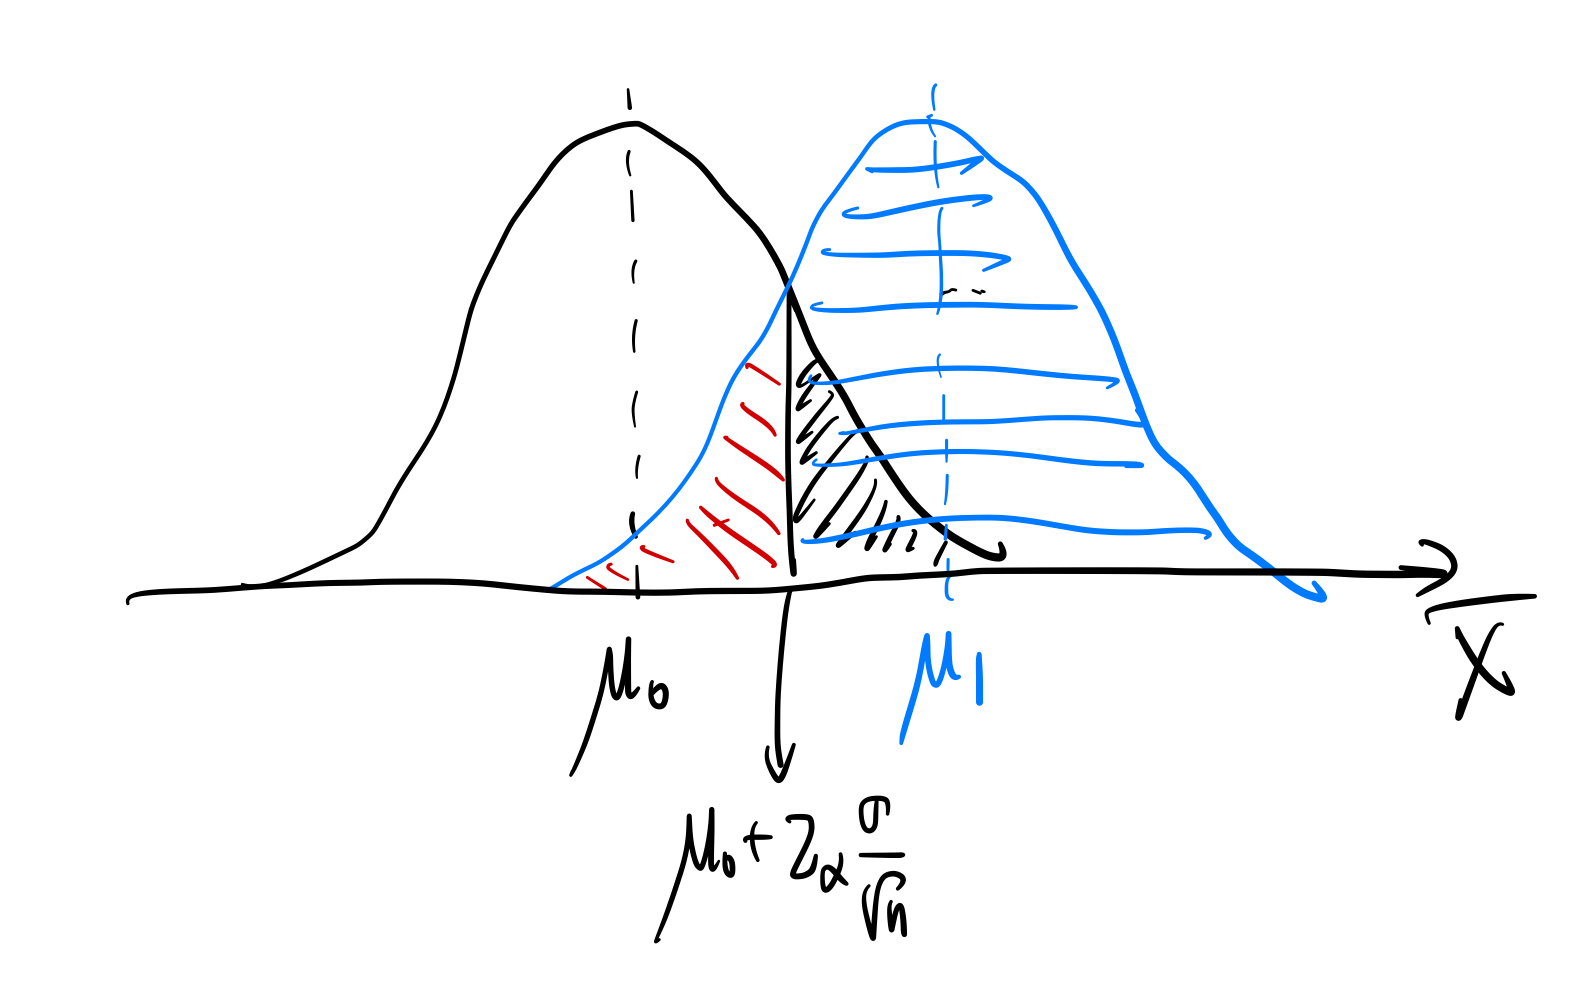
\includegraphics[width=0.8\textwidth]{figures/06-Hypothesis_testing/error_power.jpeg}
        \caption{檢定的型一錯誤率、型二錯誤率與檢定力}
        \label{fig:error_power}
    \end{figure}

    除了型一錯誤率外,我們的目的是要計算型二錯誤率(type II error rate, 常寫做 $\beta$),也就是對立假說成立下,無法拒絕虛無假說的機率。此時我們需要知道檢定統計量在對立假說成立下的抽樣分布,但我們的對立假說是 $\mu > 0$,並沒有一個明確的母體平均值。因此,我們要先設定一個對立假說下的母體平均值 $\mu_1$,以作為我們建立抽樣分布及後續計算型二錯誤率的參考。在這裡我們設定 $\mu_1 = 1$。若 $\mu = \mu_1 = 1$,$\bar{X}$ 的抽樣分布為 $\NN(\mu_1 = 1, \sigma^2/n = 1/9)$,我們將其描繪在圖 \ref{fig:error_power} 的藍色部分。型二錯誤率為對立假說成立下,無法拒絕虛無假說的機率,也就是 $\bar{X}$ 服從藍色的分布下,取值不足臨界值 0.55 的機率,即圖 \ref{fig:error_power} 中的紅色面積。這個面積的算法我們可以再次利用 z 轉換:
    \begin{align*}
        &\PP(\bar{X} < 0.55|H_1:\mu = 1) \\
        =& \PP(\bar{X} < 0.55|\bar{X} \sim \NN(1, 1/9))\\
        =& \PP\Big(\frac{\bar{X}-1}{1/3} < \frac{0.55 - 1}{1/3} \approx -1.35|\bar{X} \sim \NN(1, 1/9))\\
        =& \PP(\ZZ < -1.35) = \Phi(-1.35) \approx 0.089
    \end{align*}
    因此,我們知道當對立假說之參數取值為 $\mu = 1$ 時,檢定的型二錯誤率為 0.089。用白話來說,當母體平均實際上為 1 時,檢定「母體平均是否大於 0」卻無法拒絕虛無假說「母體平均等於 0」的機率為 0.089。這個機率越小,代表在無法拒絕虛無假說時,我們對於對立假說的信心越高。

    除了型二錯誤率以外,生醫統計上更常用的機率是它的反面:\textit{檢定力}(power)。檢定力是對立假說成立下,能夠成功拒絕虛無假說的機會。如圖\ref{tab:error_power}所示,檢定力即圖中藍色的面積(因為 $\bar{X}$ 在臨界值以上時,我們會拒絕虛無假說),因此檢定力恰等於一減去型二錯誤率。在上面的例子中,於對立假說成立且設定母體平均為 1 的情況下,該檢定的檢定力為 1-0.089 = 0.911。以白話來說,當母體平均實際上為 1 時,檢定「母體平均是否大於 0」並成功拒絕虛無假說「母體平均等於 0」的機率為 0.911。一般來說,我們希望檢定在控制型一錯誤率的前提下,檢定力能夠越大越好,我們才能有效率地判斷資料是否隱含著對立假設為真的訊息。
    
    為了瞭解什麼因素會影響檢定力,我們可以將符號重新帶回上述的所有計算,並得到單樣本母體平均值右尾檢定的檢定力公式:
    \[1-\beta = \Phi\Big(\frac{\mu_1-\mu_0}{\sigma/\sqrt{n}}-z_\alpha\Big) := \Phi\Big(\frac{\Delta}{\sigma/\sqrt{n}}-z_\alpha\Big)\]
    根據這個公式,我們可以分項探討各因素對於檢定力的導引方向:
    \begin{itemize}
        \item 效果量 $\Delta$:效果量定義為 $\mu_1-\mu_0$,即對立假說下母體平均取值與虛無假說的距離。效果量越大,檢定力也會越大。這個結果十分直覺:當對立假說下的母體平均遠大於虛無假說下的取值,那麼觀察到的樣本平均就會非常大,因此就有很大的機會拒絕虛無假說。
        \item 樣本數 $n$:當樣本數變大時,公式中的分母會變小,因此整體檢定力會變大。當樣本數變大時,資料中含有的資訊越多,我們就越有機會成功證偽虛無假說。
        \item 母體標準差 $\sigma$:當母體標準差變大時,公式中的分母會變大,因此整體檢定力會變小。母體標準差越大,代表每筆資料的資訊含量越低(可以想成測量誤差非常大,實際關於母題平均的資訊都被誤差稀釋掉了),因此成功證偽虛無假說的可能性就越低。
        \item 顯著水準(型一錯誤率) $\alpha$:通常我們不會任意調動顯著水準,但從公式可以看出,顯著水準調得越高,$z_\alpha$就會越小,因此整體檢定力就會越高。當我們把檢定的顯著水準調高,代表拒絕虛無假說的條件變得寬鬆,從而檢定力也會提高。如果用型一和型二錯誤率來看,可以知道型一錯誤率增高會讓型二錯誤率降低,反之亦然,兩者之間有一個權衡關係。
    \end{itemize}
    上述的討論中,我們雖然是用單樣本母體平均值右尾檢定作例子,但各因素對於檢定力的影響方向在各類檢定大致通用。

    檢定力公式除了可以用來計算檢定力外,另一個重要的用途是用來計算樣本數。我們一般都希望檢定的檢定力越大越好,但在檢定力公式中,母體標準差是資料的特性而無法更動,顯著水準有約定俗成的設定(通常是 0.05),而效果量則通常設定為臨床上有意義的效果差異(例如平均舒張壓下降 5 mmHg)。因此,研究者能夠隨意調動的通常只剩下樣本數,而做研究的第一步常需要了解樣本數應該要收到多少,才能夠讓檢定力達到一定水準,以求在做完研究後,如果檢定不顯著,我們還可以根據檢定力針對不顯著的結果作有信心的推論。樣本數的計算基本上就是將檢定力公式做反向推演。假設我們希望檢定力至少是 $1-\beta$(一般常設定為 0.8 或 0.9),那麼
    \[\Phi\Big(\frac{\Delta}{\sigma/\sqrt{n}}-z_\alpha\Big) \ge 1-\beta\]
    \[n \ge \Big[\frac{\sigma}{\Delta} (\Phi^{-1}(1-\beta) + z_\alpha)\Big]^2 = \Big(\frac{\sigma}{\Delta}\Big)^2(z_\alpha + z_\beta)^2\]
    一般而言實務上,考量到收進來的樣本可能會失去追蹤或是有測量失誤,因此會將樣本數設定為最低所需樣本數的倍數,例如 1.1 倍、1.25 倍等等。從這個公式可以看到,會使所需樣本數增加的因素為:母體標準差增加、所需偵測效果量降低、顯著水準上升、以及檢定力上升。這些影響方向的解釋原因和上述有關檢定力的討論類似,在這裡就不再贅述。
    
    \bigskip

    \begin{custom}{思考}
        在顯著水準維持不變的情況下,使用單尾檢定算出的樣本數應該比雙尾檢定算出的樣本數來得多還是來得少?
    \end{custom}

    \bigskip

    \begin{custom}{思考}
        若欲求比例單樣本檢定的樣本數,應該要提供那一些資訊以供計算?
    \end{custom}
    
    \begin{docexam}{(104-1醫學(一))}
        下面有關假說檢定之型一錯誤(type I error)與型二錯誤(type II error)的敘述何者正確?

        (A) 型一錯誤發生的機率加上型二錯誤發生的機率等於 1

        (B) 檢定力(power) = 1-型一錯誤的機率

        (C) 型一錯誤與型二錯誤有可能會同時發生

        (D) 固定型一錯誤的機率,增加樣本數可以降低型二錯誤發生的機率
    \end{docexam}
    
    \begin{docexam}{(107-1醫學(二))}
        進行統計檢定,當根據數據計算所得之 $p$ 值 > $\alpha$ (顯著水準)時,下列敘述何者正確?

        (A) 可以正確推翻虛無假設

        (B) 證據不足以推翻虛無假設

        (C) 可以正確接受虛無假設

        (D) 可能犯型 I 錯誤
    \end{docexam}

    % \bigskip
    
    % \begin{docexam}{(105-2醫學(一))}
    %     某麻醉科醫師想比較兩種麻醉藥物(舊藥與新藥)的效果,計畫收集採用舊藥50人及新藥50位病人在麻醉開始後至手術開始時的最小血壓值。麻醉科醫師希望可以偵測到兩組最小血壓值差距到 6 mmHg,下列何者做法可以提升統計假設檢定的檢定力 (power)?

    %     (A) 將檢定的顯著性水準由 0.05 增加至 0.1

    %     (B) 偵測到兩組最小血壓差距由 6 mmHg 降低到 3 mmHg

    %     (C) 樣本更改為收集舊藥 40 人及新藥 60 位病人

    %     (D) 樣本更改為收集舊藥 60 人及新藥 40 位病人
    % \end{docexam}
    
    \begin{docexam}{(105-1醫學(一))}
        兩種麻醉藥物死亡率差異的 $95\%$ 信賴區間為 (-0.142,0.102),若將檢定之顯著性水準由 0.05 更改為 0.01,其他條件不變下,檢定兩種麻醉藥物的死亡率是否有差異,下列敘述何者正確?

        (A) 兩種麻醉藥物的死亡率達統計顯著

        (B) 兩種麻醉藥物的死亡率未達統計顯著

        (C) 無法下結論

        (D) 此檢定的結果有可能犯下型一錯誤 (type I error)
    \end{docexam}
    
    \begin{docexam}{(104-2醫學(一))}
        下列哪一選項能夠增加統計檢定力(statistical power)?

        (A) 採用雙盲 (double-blind)

        (B) 隨機分派 (randomization)

        (C) 增加樣本數 (sample size)

        (D) 使用對照組 (control)
    \end{docexam}
    
    \begin{docexam}{(103-2醫學(一))}
        統計假說檢定(statistical hypothesis testing)時,何謂型二錯誤(type II error)?

        (A) 兩組實際上無差異,分析結果推翻虛無假說(null hypothesis)

        (B) 兩組實際上無差異,分析結果支持虛無假說

        (C) 兩組實際上有差異,分析結果推翻虛無假說

        (D) 兩組實際上有差異,分析結果支持虛無假說
    \end{docexam}
    
    \begin{docexam}{(103-2醫學(一))}
        一項研究探討中學生現在近視的比例 (m0) 是否高於 10 年前,如果 10 年前中學生的近視比例是 45\%,下列有關虛無假設 (null hypothesis, H0) 與對立假設 (alternative hypothesis, HA) 的敘述,何者正確?

        (A) H0: m0 = 0 vs HA: m0 $\ne$ 0

        (B) H0: m0 = 0.45 vs HA: m0 $\ne$ 0.45

        (C) H0: m0 $\ge$ 0.45 vs HA: m0 < 0.45

        (D) H0: m0 $\le$ 0.45 vs HA: m0 > 0.45
    \end{docexam}
    
    \begin{docexam}{(103-1醫學(一))}
        下列有關檢力(power)的敘述,何者正確?

        (A) 降低顯著水準,例如從 0.05 變成 0.01,檢力將變大

        (B) 如果對立假設的平均值,比預期更遠離虛無假設的平均值,則檢定的檢力將增加

        (C) 若觀測值的標準差增加,則檢力增加

        (D) 若樣本數減少,則檢力增加
    \end{docexam}
    
    \begin{docexam}{(101-2醫學(一))}
        在統計推論做雙尾檢定時,經計算得 $p$ 值為 0.04,若其他條件不變,改做單尾檢定,其 $p$ 值會有何種變化?

        (A) 變大

        (B) 變小

        (C) 如果變項是常態分布的情況下會變大,若不是則變小

        (D) 如果變項是常態分布的情況下會變小,若不是則變大
    \end{docexam}
    
    \begin{docexam}{(101-2醫學(一))}
        有關統計檢定,下列哪一項敘述錯誤?

        (A) 統計的 Power 係指可正確判斷新治療方式有效的機率

        (B) 統計的 Type I error 係指新治療方式無效,卻被判定為有效的機率

        (C) 統計的 Type I error 係指新治療方式無效,卻被判定為有效的機率

        (D) 統計的信賴水準 ($1-\alpha$) 係指新治療方式無效,可被正確判斷的機率
    \end{docexam}
    
    \begin{docexam}{(101-1醫學(一))}
        某小型臨床試驗評估一個新化療治療淋巴癌的療效,若事實上此新化療有比較好的療效,但本研究沒發現顯著的五年存活率差異,無法偵測此新治療效果的原因為何?

        (A) 檢力(power)太大

        (B) 抽樣誤差

        (C) 型一誤差(type I error)

        (D) 型二誤差(type II error)
    \end{docexam}
    
    \begin{docexam}{(101-1醫學(一))}
        甲醫院手術治療某種疾病,抽樣100個病人有80個治療成功,成功率的 95\% 信賴區間 (95\% confidence interval) 為 (0.72,0.88)。如果一般全國平均治療這種病人的成功率為 90\%,我們想以此資料來做假說檢定,檢定甲醫院治療此病成功率是否比 90\% 低,顯著水準設為 $\alpha$ = 0.05,下列何者正確?

        (A) 無法推翻虛無假說,結論是甲醫院的治療成功率與 95\% 一樣

        (B) 推翻虛無假說,結論是甲醫院的治療成功率比 90\% 低

        (C) 無法推翻虛無假說,結論是甲醫院的治療成功率比 90\% 低

        (D) 推翻虛無假說,結論是甲醫院的治療成功率與 90\% 一樣
    \end{docexam}
    
    \begin{docexam}{(100-1醫學(一))}
        當一個研究者結論未能偵測出顯著的效應,下列何者的誤差和研究者的結論有關聯?

        (A) 因為樣本數太小,此結論錯誤的可能性很低

        (B) 犯下第二誤差的可能性很小

        (C) 第一誤差的機率大於0.05

        (D) 犯下第二誤差的可能性很大
    \end{docexam}
    
    \begin{docexam}{(108-1醫學(二))}
        一研究想比較抽菸者與非抽菸者的血膽固醇濃度,下列敘述何者錯誤?

        (A) 檢定時犯下型一錯誤 (type I error) 的機率,即為研究者設定的顯著水準

        (B) 若顯著水準不變,欲增加統計檢定力,可以增加樣本數

        (C) 型一錯誤是抽菸者與非抽菸者的血膽固醇濃度沒差異,但檢定時卻誤判有差異的情形

        (D) 型一錯誤加型二錯誤的機率和為 $1$
    \end{docexam}
    
    \begin{docexam}{(108-2醫學(二))}
        統計假說檢定 (statistical hypothesis testing) 時,何謂型一錯誤 (type I error)?

        (A) 兩組實際上無差異,分析結果推翻虛無假說 (null hypothesis) 

        (B) 兩組實際上無差異,分析結果支持虛無假說 (null hypothesis) 

        (C) 兩組實際上有差異,分析結果推翻虛無假說 (null hypothesis) 

        (D) 兩組實際上有差異,分析結果支持虛無假說 (null hypothesis) 
    \end{docexam}
    
    \begin{docexam}{(108-2醫學(二))}
        有關單尾與雙尾假說檢定的敘述,下列何者正確?

        (A) 單尾與雙尾假說檢定的 $p$ 值算法相同

        (B) 相對於雙尾假說檢定,單尾假說檢定比較不易拒絕虛無假說

        (C) 單尾與雙尾假說檢定的顯著水準 ($\alpha$) 相同 

        (D) 相對於雙尾假說檢定,單尾假說檢定比較常被使用
    \end{docexam}

    \begin{docexam}{(112-1醫學(二))}
        醫療檢測數據呈現明顯右偏分布,下列何組指標最適合測量此群資料之集中與分散狀況?

        (A) 平均值,標準差

        (B) 平均值,標準誤

        (C) 中位數,四分位距

        (D) 中位數,全距
    \end{docexam}
    